\documentclass[article]{jss}
\usepackage{amsmath}
\usepackage[utf8]{inputenc}
\usepackage{graphicx}
\usepackage{natbib}
\usepackage{enumerate}
\usepackage{dsfont}

%%%%%%%%%%%%%%%%%%%%%%%%%%%%%%
%% declarations for jss.cls %%%%%%%%%%%%%%%%%%%%%%%%%%%%%%%%%%%%%%%%%%
%%%%%%%%%%%%%%%%%%%%%%%%%%%%%%

%% almost as usual
\author{Brendon J. Brewer\\The University of Auckland\And 
        Daniel Foreman-Mackey\\University of Washington}
\title{\pkg{DNest4}: Diffusive Nested Sampling in
\proglang{C++} and \proglang{Python}}

%% for pretty printing and a nice hypersummary also set:
\Plainauthor{Brendon J. Brewer, Daniel Foreman-Mackey} %% comma-separated
\Plaintitle{DNest4: An implementation of Diffusive Nested Sampling in
C++11 and Python} %% without formatting
\Shorttitle{\pkg{DNest4}: Diffusive Nested Sampling} %% a short title (if necessary)

%% an abstract and keywords
\Abstract{In probabilistic (Bayesian) inferences, we typically want to compute
properties of the posterior distribution, describing knowledge of
unknown quantities in the context of a particular dataset and the assumed
prior information. The marginal likelihood (also known as the ``evidence'')
is a key quantity in Bayesian model averaging. The Diffusive Nested Sampling algorithm, a variant of Nested Sampling, is a powerful tool for generating
posterior samples and estimating marginal likelihoods. It is effective at
solving complex problems including many where the posterior distribution is
multimodal or has strong dependencies between variables. The key requirement
is that the likelihood function be fast to evaluate.
\pkg{DNest4} is an open source (MIT licensed),
multi-threaded implementation of this algorithm in
modern \proglang{C++} (specifically, \proglang{C++11}),
along with associated utilities including: i)
a \pkg{Python} package allowing basic use without \proglang{C++} coding;
ii) \pkg{RJObject}, a class template for finite mixture models;
iii) Experimental support for models implemented in \proglang{Julia}; and
iv) An experimental \proglang{Python} tool to
generate \pkg{C++} code from a model specification.
In this paper we demonstrate \pkg{DNest4} usage through examples including
simple Bayesian data analysis, finite mixture models, and Approximate
Bayesian Computation (ABC).
}

\Keywords{bayesian inference, markov chain monte carlo,
metropolis algorithm, bayesian computation, nested sampling, \proglang{c++11},
\proglang{python}}
\Plainkeywords{bayesian inference, markov chain monte carlo,
metropolis algorithm, bayesian computation, nested sampling, c++11, python} %% without formatting
%% at least one keyword must be supplied

%% publication information
%% NOTE: Typically, this can be left commented and will be filled out by the technical editor
%% \Volume{50}
%% \Issue{9}
%% \Month{June}
%% \Year{2012}
%% \Submitdate{2012-06-04}
%% \Acceptdate{2012-06-04}

%% The address of (at least) one author should be given
%% in the following format:
\Address{
  Brendon J. Brewer\\
  Department of Statistics\\
  The University of Auckland\\
  Private Bag 92019\\
  Auckland, 1142\\
  New Zealand\\
  E-mail: \email{bj.brewer@auckland.ac.nz}\\
  URL: \url{https://www.stat.auckland.ac.nz/~brewer/}
}

\newcommand{\params}{\theta}
\newcommand{\data}{D}
\newcommand{\dobs}{D_{\rm obs}}

\begin{document}
\maketitle

%% Need this after the abstract
%\setlength{\parindent}{0pt}
%\setlength{\parskip}{8pt}

\section{Introduction}
Bayesian inference, where probability theory is used to describe degrees of
logical implication or subjective certainty, provides a powerful general basis
for data analysis \citep{ohagan, sivia}. The result of such
an analysis is typically
posterior probabilities of various hypotheses, or (more specifically)
a joint posterior probability distribution for the values of unknown
parameters.

In a very compact (but standard) notation, the posterior
posterior distribution for parameters $\params$ given data $\data$, within
the context of prior information $M$, is
\begin{align}
p(\params | \data, M) &=
\frac{p(\params | M)p(\data | \params, M)}{p(\data | M)}
\end{align}
or
\begin{align}
\textnormal{posterior} &=
\frac{\textnormal{prior} \times \textnormal{likelihood}}
     {\textnormal{marginal likelihood}}.
\end{align}

If prior information $I$ (hereby dropped)
implies a set of possible `models' $\{M_i\}$,
rather than a single one $M$, the posterior model probabilities are given by
\begin{align}
P(M_i | \data) &=
\frac{P(M_i)p(\data | M_i)}{\sum_j P(M_j)p(\data | M_j)}
\end{align}
where
\begin{align}
p(\data | M_j) &= \int p(\theta_j | M_j)p(\data | \theta_j, M_j) \, d\theta_j
\end{align}
is the marginal likelihood of model $j$. This kind of calculation is often
called ``model selection'' or (more accurately) ``model averaging''.

When discussing computational matters, the prior distribution for parameters
is
often written $\pi(\theta)$, the likelihood $L(\theta)$,
and the marginal likelihood $Z$. A popular alternative name for the marginal
likelihood, which emphasizes its role in Bayesian model averaging,
is the ``evidence''.

Nested Sampling \citep[NS;][]{skilling} is a Monte Carlo method whose main
aim is to calculate $Z$. However, it can also be used to generate samples
to represent the posterior distribution $\pi(\theta)L(\theta)/Z$, or
any other distribution proportional to
$\pi(\theta)\Phi\left[L(\theta)\right]$ where $\Phi$ is any monotonic function.
This latter property makes NS particularly useful for statistical mechanics
calculations \citep{2009arXiv0906.3544P, 2015arXiv150303404B}, where the
``canonical'' family of distributions proportional to
$\pi(\theta)L(\theta)^\beta$ is of interest (and $L(\theta)$ is identified as
$\exp(-\textnormal{energy})$). NS is particularly efficient for this, since
only a single run (which explores regions of higher and higher $L$)
is required, and different canonical
distributions can be obtained by re-weighting the output points.

A defining feature of NS is that it works with a sequence of
{\em constrained prior} distributions, proportional to $\pi$ but
restricted to regions of the parameter space where $L(\theta)$
is above some threshold $\ell$:
\begin{align}
p(\theta; \ell) &=
\frac{\pi(\theta)\mathds{1}\left[L(\theta) > \ell\right]}{X(\ell)}
\label{eqn:constrained_prior}
\end{align}
where
\begin{align}
X(\ell) &= \int \pi(\theta) \mathds{1}\left[L(\theta) > \ell\right] \, d\theta
\end{align}
is the amount of prior mass which has likelihood greater than $\ell$.
In the standard NS framework, the sequence of $\ell$ values is selected
so that $X(\ell)$ shrinks by a factor $\approx e^{-1/N}$ per iteration, where
$N$ is the number of particles used.

Sampling from the constrained priors (Equation~\ref{eqn:constrained_prior})
is required, and Markov Chain Monte Carlo (MCMC) is a popular method of doing
this, although alternatives exist \citep[e.g.][]{multinest, handley}.

Diffusive Nested Sampling \citep[DNS][]{dnest} is an alternative to NS for
problems where MCMC is the only viable sampling method. DNS is based on the
Metropolis algorithm. DNS evolves a point in the parameter space, along with
an integer index variable $j$,
to explore the following joint distribution:
\begin{align}
p(\theta, j) &= p(j)p(\theta | j)\\
&= w_j \times
\frac{\pi(\theta)\mathds{1}\left[L(\theta) > \ell_j\right]}{X(\ell_j)}.
\label{eqn:target_distribution}
\end{align}
where the $\{\ell_j\}$ are a sequence of increasing likelihood thresholds
or {\em levels}, and
$\ell_0 = 0$, and $\{w_j\}$ is the marginal distribution for $j$.
The marginal distribution for $\theta$ is then a {\em mixture} of
constrained priors:
\begin{align}
p(\theta) &=
\pi(\theta)\sum_{j=0}^{j_{\rm max}}
\frac{w_j\mathds{1}\left[L(\theta) > \ell_j\right]}{X(\ell_j)}.
\label{eqn:mixture_of_constrained_priors}
\end{align}

DNS has been applied several times in astrophysics
\citep[e.g.][]{2014MNRAS.445.3055P, 2015ApJ...810...66H, 2015MNRAS.448.3206B}
and was recently used in a biological application \citep{salmonella}.

There are several ways of using \pkg{DNest4}. After installing the software
(Section~\ref{sec:installation}), you can implement a model as
a \proglang{C++} class
(Section~\ref{sec:models}) and compile it to create an executable file
to run \pkg{DNest4} on that problem. This method offers full control over the
design of your class, and allows the opportunity (for example) to optimise
performance by preventing a full re-computation of the log-likelihood when
only a small subset of the parameters were changed.

Similarly, the \proglang{Python}
bindings (Section~\ref{sec:python_bindings}) allow you
to specify a model class in \proglang{Python}, and run \pkg{DNest4} entirely
in the \proglang{Python} interpreter without having to invoke the \proglang{C++}
compiler.

\section{Markov Chain Monte Carlo}\label{sec:mcmc}
DNS is build upon the Metropolis-Hastings algorithm.
In this algorithm, the acceptance probability $\alpha$
is given by
\begin{align}
\alpha &= \min\left(1,
\frac{q(\params'|\params)}{q(\params | \params')}
\frac{\pi(\params')}{\pi(\params)}\frac{L(\params')}{L(\params)}
\right)
\end{align}
where $q(\theta' | \theta)$ is the proposal distribution used to generate
a new position $\theta'$ from the current position $\theta$. Often,
$q$ is {\em symmetric} so the $q$ terms cancel in the acceptance probability.

In DNS, the target distribution is not the posterior but rather
the joint distribution in Equation~\ref{eqn:target_distribution}.
Moves of $\theta$ are done keeping $j$ fixed, so we only need
to consider the Metropolis acceptance probability for fixed $j$,
i.e. with respect to a single constrained prior like
Equation~\ref{eqn:constrained_prior}.
Hence, the appropriate acceptance probability
for a proposed move from $\theta$ to $\theta'$ is
\begin{align}
\alpha &= \min\left[1,
\frac{q(\params'|\params)}{q(\params | \params')}
\frac{\pi(\params')}{\pi(\params)}
\mathds{1}\left(L(\params') > \ell_j\right)
\right]
\label{eqn:log_hastings}
\end{align}
where $\ell_j$ is the likelihood threshold for level $j$.

For convenience later on, we 
separate the prior and proposal-related terms from
the likelihood-related term, and write the former as
\begin{align}
H = \frac{q(\params'|\params)}{q(\params | \params')}
\times \frac{\pi(\params')}{\pi(\params)}
\end{align}
so the acceptance probability becomes
\begin{align}
\alpha &= \min\left[1,
H\times
\mathds{1}\left(L(\params') > \ell_j\right)
\right]
\end{align}


%The \pkg{DNest4} \code{Sampler} class handles the likelihood check,
%while the \code{perturb(DNest4::RNG\&)} member function handles the
%rest of the terms. The value returned from \code{perturb(DNest4::RNG\&)}
%must be
%for your problem.



%\subsection{Diffusive Nested Sampling}



\section{Dependencies and installation}\label{sec:installation}

\subsection{Unix-like operating systems}
The following instructions apply to Unix-like operating systems such as
GNU/Linux, Mac OS X, and FreeBSD.
\pkg{DNest4} can be obtained from the \pkg{git} repository located at
\begin{center}
{\tt https://github.com/eggplantbren/DNest4/}\\
\end{center}
and is licensed under the
MIT license. To obtain and compile \pkg{DNest4},
you require \pkg{git} and a recent version of the GNU
\proglang{C++} compiler, \pkg{g++}. The \proglang{Python}
packages \pkg{NumPy}, \pkg{matplotlib},
\pkg{Pandas}, and \pkg{Cython} are also needed.
To download and compile \pkg{DNest4}
the following steps are sufficient:
\begin{CodeChunk}
\begin{CodeInput}
git clone https://github.com/eggplantbren/DNest4
cd DNest4/code
make
cd ../python
python setup.py install
\end{CodeInput}
\end{CodeChunk}

\subsection{Microsoft Windows}


%\subsection{Multithreading}

\section{Running models}


\begin{figure}
\centering
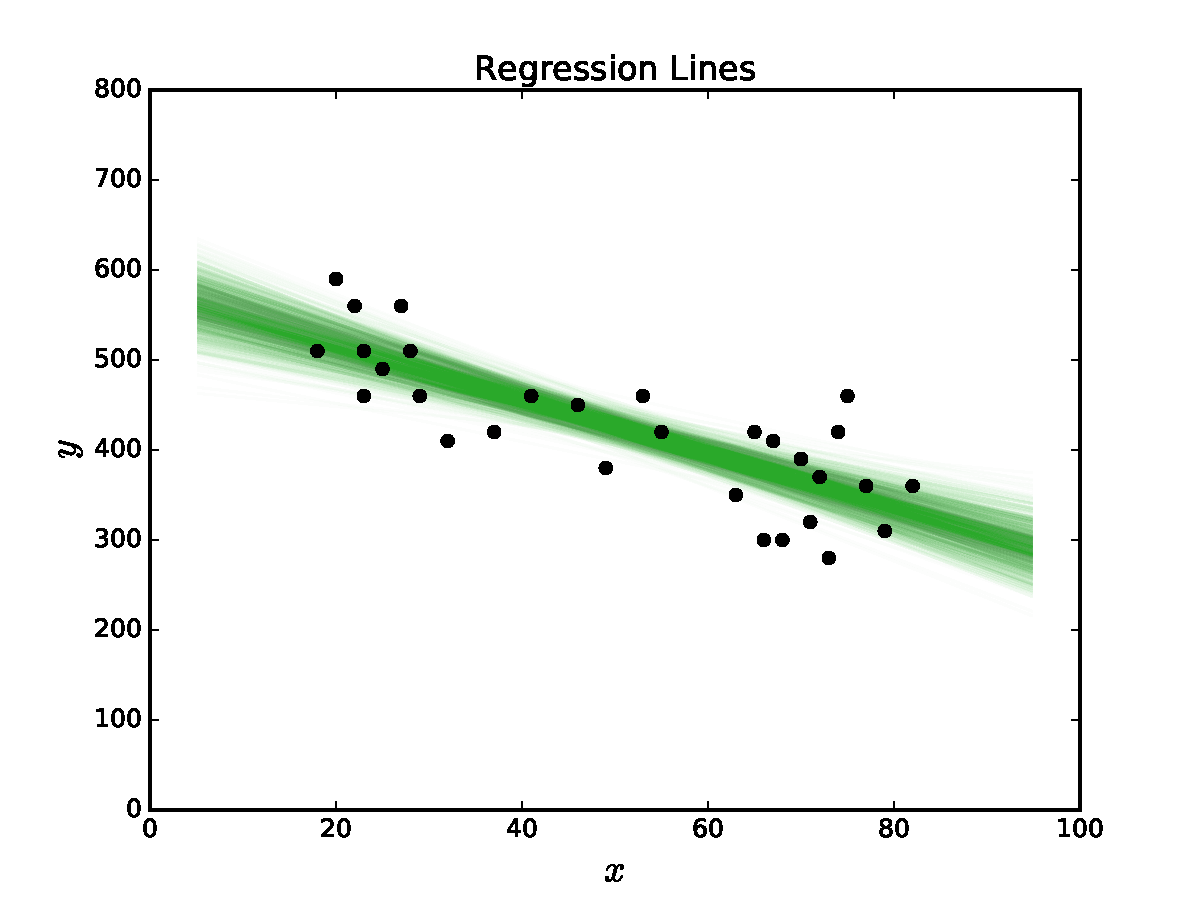
\includegraphics[width=0.8\textwidth]{figures/regression_lines.pdf}
\caption{Regression lines drawn from the posterior.
\label{fig:regression_lines}}
\end{figure}

\subsection{Options}
A plain-text file called OPTIONS resides in the directory from which you
execute a run.

Additional options are available on the command line. These are
described in Appendix~\ref{sec:command_line_options}.

\section{Implementing models}\label{sec:models}
The ``classic'' method of implementing models in \pkg{DNest4} is by
writing a \proglang{C++} class, an object of which represents a
point in your parameter space.
To demonstrate, consider a simple linear regression situation where the
sampling distribution is
\begin{align}
y_i | m, b, \sigma &\sim \textnormal{Normal}(mx_i + b, \sigma^2)
\end{align}
and the priors are
\begin{align}
m &\sim \textnormal{Normal}(0, 1000^2)\\
b &\sim \textnormal{Normal}(0, 1000^2)\\
\ln\sigma &\sim \textnormal{Uniform}(-10, 10)
\end{align}
These are naive diffuse priors and we do not claim any special status for them.

To run \pkg{DNest4} on any particular problem, such as this linear regression
example, the user needs to define a \proglang{C++} class to specify the
model. Specifically, an object of the class represents a point in the
model's parameter space. Member functions are defined which generate
the object's parameters from the prior, make proposal steps, evaluate the
likelihood, and so on. The sampler calls these member functions while
executing a run.

For the simple linear regression example, we will call the class
{\tt StraightLine}. The member variables representing the
unknown parameters are defined in the header file {\tt StraightLine.h}:

\begin{CodeChunk}
\begin{CodeInput}
class StraightLine
{
    private:
        double m, b, sigma;
};
\end{CodeInput}
\end{CodeChunk}

The class must also define and implement the following member functions:
\begin{enumerate}[(i)]
\item \code{void from\_prior(DNest4::RNG\& rng)}, which generates parameter
        values from the prior;
\item \code{double perturb(DNest4::RNG\& rng)}, which proposes a
        change to the parameter values, and returns $\ln(H)$ as defined in
        Equation~\ref{eqn:log_hastings};
\item \code{double log\_likelihood() const}, which evaluates the log of
        the likelihood function;
\item \code{void print(std::ostream\& out) const}, which prints parameters of
        interest to the given output stream; and
\item \code{std::string description() const}, which returns a \proglang{C++}
        string naming the parameters printed by \code{print(std::ostream\&) const}.
        This string is printed (after a comment character \#) at the top of
        the output file.
\end{enumerate}

%%\subsection{generate}

%\section{Python package}

%% Assign to DFM

%\section{Examples}
% Reasonably simple examples

The member function used to generate straight line parameters from the
prior is:

\begin{CodeChunk}
\begin{CodeInput}
void StraightLine::from_prior(DNest4::RNG& rng)
{
   // Naive diffuse prior
   m = 1E3*rng.randn();
   b = 1E3*rng.randn();

   // Log-uniform prior
   sigma = exp(-10.0 + 20.0*rng.rand());
}
\end{CodeInput}
\end{CodeChunk}

This generates $m$, $b$, and $\sigma$ from their joint prior. In this case,
the priors are all independent, so this reduces to generating the parameters
each from their own prior distribution. For convenience, the \code{RNG} object
has \code{rand()} and \code{randn()} member functions to generate from
a Uniform$(0,1)$ and Normal$(0,1)$ distribution respectively.

After generating the parameters from the prior, another member function
\code{calculate\_mu()} is called, which computes the model prediction
$mx_i + b$ for each data point.

The \code{perturb} member function for the straight line model is:
\begin{CodeChunk}
\begin{CodeInput}
double StraightLine::perturb(DNest4::RNG& rng)
{
	double log_H = 0.0;

	// Proposals explore the prior
	// For normal priors I usually use the hastings factor to do it
	int which = rng.rand_int(3);
	if(which == 0)
	{
		log_H -= -0.5*pow(m/1E3, 2);
		m += 1E3*rng.randh();
		log_H += -0.5*pow(m/1E3, 2);
	}
	else if(which == 1)
	{
		log_H -= -0.5*pow(b/1E3, 2);
		b += 1E3*rng.randh();
		log_H += -0.5*pow(b/1E3, 2);
	}
	else
	{
		// Usual log-uniform prior trick
		sigma = log(sigma);
		sigma += 20.0*rng.randh();
		DNest4::wrap(sigma, -10.0, 10.0);
		sigma = exp(sigma);
	}

	return log_H;
}
\end{CodeInput}
\end{CodeChunk}

This first chooses a random integer from $[0, 3)$ using the
\code{rand\_int(int)} member function of the \code{DNest4::RNG} class.
This determines which of the three parameters is modified.


When implementing a model class, it is imperative that the
\code{from\_prior(DNest4::RNG\&)} and \code{perturb(DNest4::RNG\&)}
member functions be consistent with each other. One technique
for verifying this is to sample the prior for a long time
(by setting the maximum number of levels to 1) and inspect
{\tt sample.txt} to ensure that each parameter is exploring
the correct distribution.

The log-likelihood code is:
\begin{CodeChunk}
\begin{CodeInput}
double StraightLine::log_likelihood() const
{
    // Grab the dataset
    const std::vector<double>& x = Data::get_instance().get_x();
    const std::vector<double>& y = Data::get_instance().get_y();

    // Variance
    double var = sigma*sigma;

    // Conventional gaussian sampling distribution
    double log_L = 0.0;
    double mu;
    for(size_t i=0; i<y.size(); ++i)
    {
        mu = m*x[i] + b;
        log_L += -0.5*log(2*M_PI*var) - 0.5*pow(y[i] - mu, 2)/var;
    }

    return log_L;
}
\end{CodeInput}
\end{CodeChunk}
The dataset is assumed to be accessible inside this function. In the
regression example, this is achieved by having a
\code{Data} class to represent
datasets. Since there will usually only be one dataset,
the {\em singleton pattern} (a class of which there is one instance
accessible from anywhere) is recommended.

The print and description functions are very simple:
\begin{CodeChunk}
\begin{CodeInput}
void StraightLine::print(std::ostream& out) const
{
    out<<m<<' '<<b<<' '<<sigma;
}

std::string StraightLine::description() const
{
    return std::string("m, b, sigma");
}

\end{CodeInput}
\end{CodeChunk}

\section{Approximate Bayesian Computation}
Nested Sampling can be used to solve ``Approximate Bayesian Computation''
problems elegantly and efficiently.

Approximate Bayesian Computation (ABC), also known as likelihood-free inference,
is a set of Monte Carlo techniques for approximating a posterior distribution
without having to evaluate the likelihood function $L(\theta)$.

. Instead, the ability to
generate simulated data sets from the sampling distribution is required.
Since a sampling distribution must be specified, it is not the assumption of
a specific likelihood that is avoided (indeed, a sampling distribution and
a data set imply a particular likelihood function), rather that we cannot
evaluate it cheaply as a function of $\params$ and $\data$.

All Bayesian updating conditions on the truth of a proposition. We sometimes
speak and use notation as if we're conditioning on the value of a variable, for
example by writing the posterior distribution as $p(\params | \data)$. However,
this is shorthand for $p(\params | \data = \dobs)$. In the prior state of
knowledge, the proposition $(\data = \dobs)$ could have been either true or
false, but in the posterior state of knowledge it is definitely true.
In the case of ``continuous data'' (really a continuous {\it space of
possibilities for the data before we learned it}) we're conditioning on a
proposition like $(\data \in [\dobs, \dobs+\epsilon])$ and implicitly
taking the limit $\epsilon \to 0$.

\begin{table}[ht!]
\centering
\small
\begin{tabular}{|l|l|l|}
\hline
Bayesian computation		&		Statistical mechanics		&		ABC\\
\hline
Parameter space	$\Theta$	&		Phase space	$\Omega$ 			& Product space $\Theta \times \mathcal{D}$\\
Posterior $p(\params | D,I)$   &  Canonical distribution $p(\boldsymbol{x}; T)$     & \\ 
Marginal likelihood $P(D|I)$	&	Partition function $Z(T)$	&   Marginal likelihood $p(D\in | I)$\\
\hline
\end{tabular}
\caption{\it The relationship between standard Bayesian computation, statistical
mechanics, and ABC. In each case Monte Carlo methods are used to calculate
integrals over a space. In standard Bayesian computation, it is the parameter
space of a model that is usually of interest, whereas in ABC it is the space
of possible parameter values {\it and} data sets.
\label{tab:relation}}
\end{table}


\begin{figure}[ht!]
\centering
\includegraphics[scale=0.5]{figures/joint.pdf}
\caption{\it The joint prior for parameters $\params$ and data $\data$.
\label{fig:joint}}
\end{figure}

The main challenges associated with ABC are:
\begin{enumerate}[(a)]
\item The choice of summary statistics
\item The choice of distance function
\item How to choose the value of $\epsilon$, or how to change it as a run
progresses
\item How to achieve good mixing.
\end{enumerate}
Challenges 1 and 2 are Bayesian in nature, i.e. they relate to the very
definition of the posterior distribution and are well defined independent of
the fact that we are going to use a Monte Carlo method to compute the
results. On the other hand, challenges 3 and 4 are about the computational implementation.

\section{Parameterising the data space}
In standard MCMC-based ABC, proposal moves are made by first proposing a
change to the parameters (from $\params$ to $\params'$), and then generating
a mock dataset $\data'$ from $p(\data | \params')$. As a Metropolis proposal
for exploring the product space $\Theta \times \mathcal{D}$ this is a very
aggressive choice, since the proposed value of the
dataset $\params'$ is likely to be very different from the previous one.
One of the most elementary pieces of advice we receive when learning the
Metropolis algorithm is to be careful about how ambitious our proposal
distributions are, since tiny and huge proposal moves are both very
inefficient. The performance of MCMC-based ABC can therefore be improved by
alternative choices of proposal distribution.

In some cases, we might be able to find efficient proposal distributions for exploring $\Theta \times \mathcal{D}$ by having insight into the particular
problem we're working on. However, there are also techniques that are
completely general in that they should work on any ABC-type problem.

Consider the process of generating a mock dataset. Whatever else is involved,
this process will involve calls to an underlying random number generator.
Perhaps a function {\tt rand()}, generating variables from a Uniform(0, 1)
distribution, is called $n$ times in the course of generating a dataset.
Usually, the simulation process has the property that, if $\theta'$ is
close to $\theta$, then the same sequence of random numbers returned by
{\tt rand()} would produce a dataset $\data'$ that is very similar to $\data$.
This suggests an alternative parameterisation of
the product space $\Theta\times\mathcal{D}$: instead of using the one that
naturally describes the data, we can use a coordinate system defined by
$\theta$ together with $\{u_1, ..., u_n\}$, the $n$ uniform random numbers
used to construct a mock dataset.

In this alternative coordinate system, a proposed move
to change $\params$ while keeping
$\{u_i\}$ fixed results in a proposed new dataset that is similar to the
previous one, assuming the change to $\params$ is small. The standard procedure
of generating an entirely new mock dataset each step is now viewed as a
proposal where $\params$ is moved {\it and all of the $u_i$ coordinates are
re-generated from their iid uniform prior}.

\subsection{Python Bindings}\label{sec:python_bindings}



\section*{Acknowledgements}
It is a pleasure to thank Anna Pancoast (Harvard),
Ewan Cameron (Oxford), David Hogg (NYU), and Daniela Huppenkothen (NYU)
for valuable discussions. BJB was supported by a Marsden Fast-Start grant
from the Royal Society of New Zealand.

\begin{thebibliography}{99}
\bibitem[Baldock et al.(2015)]{2015arXiv150303404B} Baldock, R.~J.~N., 
P{\'a}rtay, L.~v.~B., Bart{\'o}k, A.~P., Payne, M.~C., Cs{\'a}nyi, G.\ 
2015.\ Determining pressure-temperature phase diagrams of materials.\ ArXiv 
e-prints arXiv: 1503.03404. 

\bibitem[\protect\citeauthoryear{Brewer, P{\'a}rtay,
\& Cs{\'a}nyi}{2011}]{dnest} Brewer B.~J., P{\'a}rtay L.~B., Cs{\'a}nyi G., 2011,
Statistics and Computing, 21, 4, 649-656. arXiv:0912.2380

\bibitem[Brewer and Donovan(2015)]{2015MNRAS.448.3206B} Brewer, B.~J., Donovan, C.~P.\ 2015.\ Fast Bayesian inference for exoplanet discovery in radial velocity data.\ Monthly Notices of the Royal Astronomical Society 448, 3206-3214. 

\bibitem[Caticha(2008)]{caticha} Caticha, A.\ 2008.\ Lectures 
on Probability, Entropy, and Statistical Physics.\ ArXiv e-prints 
arXiv:0808.0012.

\bibitem[Dybowski et al(2015)]{salmonella}
Dybowski, Richard, et al. Single passage in mouse organs enhances the survival and spread of Salmonella enterica. Journal of The Royal Society Interface 12.113 (2015): 20150702.

\bibitem[\protect\citeauthoryear{Feroz, Hobson,
\& Bridges}{2009}]{multinest} Feroz F., Hobson M.~P., Bridges M., 2009, MNRAS, 398, 1601

\bibitem[Handley et al.(2015)]{2015MNRAS.453.4384H} Handley, W.~J., Hobson, M.~P., Lasenby, A.~N.\ 2015.\ POLYCHORD: next-generation nested sampling.\ Monthly Notices of the Royal Astronomical Society 453, 4384-4398. 

\bibitem[Huppenkothen et al.(2015)]{2015ApJ...810...66H} Huppenkothen, D., Brewer, B.~J., Hogg, D.~W., Murray, I., Frean, M., Elenbaas, C., Watts, A.~L., Levin, Y., van der Horst, A.~J., Kouveliotou, C.\ 2015.\ Dissecting Magnetar Variability with Bayesian Hierarchical Models.\ The Astrophysical Journal 810, 66. 

\bibitem[\protect\citeauthoryear{O'Hagan and Forster}{2004}]{ohagan}
O'Hagan, A., Forster,~J., 2004, Bayesian inference. London: Arnold.

\bibitem[Pancoast et al.(2014)]{2014MNRAS.445.3055P} Pancoast, A., Brewer, B.~J., Treu, T.\ 2014.\ Modelling reverberation mapping data - I. Improved geometric and dynamical models and comparison with cross-correlation results.\ Monthly Notices of the Royal Astronomical Society 445, 3055-3072.

\bibitem[\protect\citeauthoryear{Sivia and Skilling}{2006}]{sivia} Sivia, 
D.~ S., Skilling, J., 2006, Data Analysis: A Bayesian Tutorial, 2nd 
Edition, Oxford University Press

\bibitem[P{\'a}rtay et al.(2009)]{2009arXiv0906.3544P} P{\'a}rtay, L.~B., 
Bart{\'o}k, A.~P., Cs{\'a}nyi, G.\ 2009.\ Efficient sampling of atomic 
configurational spaces.\ ArXiv e-prints arXiv: 0906.3544. 

\bibitem[\protect\citeauthoryear{Skilling}{2006}]{skilling} Skilling, J., 2006, Nested Sampling for General Bayesian Computation, Bayesian Analysis 4, pp. 833-860.

\end{thebibliography}

\appendix
\section{Command Line Options}\label{sec:command_line_options}
The following command line options are available.\\

\code{-o <filename>}\\
This option loads the \pkg{DNest4} options from the specified file, allowing
an alternative to the default OPTIONS.\\

\code{-s <seed>}\\
This seeds the random number generator with the specified value. If unspecified, the system time is used.\\

\code{-d <filename>}\\
Load data from the specified file, if required.\\

\code{-c <value>}\\
Standard DNS creates levels with a volume ratio of approximately
$e\approx 2.71828$. To use a different value, such as 10, use this option.\\

\code{-t <num\_threads>}\\
Run on the specified number of threads. The default is 1.

\end{document}

